\documentclass[hyperref={pdfpagemode=FullScreen}, aspectratio=169, 10pt]{beamer}

\usetheme[progressbar=frametitle]{metropolis}
\usepackage{appendixnumberbeamer}

\usepackage{booktabs}
\usepackage[scale=2]{ccicons}

\usepackage{pgfplots}
\usepgfplotslibrary{dateplot}

\usepackage{xspace}
\newcommand{\themename}{\textbf{\textsc{metropolis}}\xspace}

% pifont has dingbats and funny symbols
\usepackage{pifont}
\newcommand{\cmark}{\ding{51}}%
\newcommand{\xmark}{\ding{55}}%

% Tikz stuff
\usepackage{tikz}
\usepackage{tikzpeople}

% graphics
\usepackage{graphicx}
\graphicspath{ {assets/} }

% plotting stuff
\usepackage{pgfplots}
\pgfplotsset{compat=1.18}
\usetikzlibrary{intersections,decorations.markings}

% cryptography stuff
\usepackage[operators, sets]{cryptocode}

\newcommand{\plotcurve}[3][thick, every plot/.style={smooth}]{
  % plot curve y^2 = x^3 + a x + b in range [-3,3]^2
  % parameter 1 (optional): style options for curve (color, etc)
  % parameter 2: curve parameter a
  % parameter 3: curve parameter b
  \draw[gray] (-3,-3) rectangle (3,3);
  \draw[->,>=latex,gray] (-3,0) -- (3,0);
  \draw[->,>=latex,gray] (0,-3) -- (0,3);
  \draw[name path=curve, #1] plot[id=curve#2#3, raw gnuplot] function {
    f(x,y) = y**2 - x**3 - #2*x - #3;
    set xrange [-3:3];
    set yrange [-3:3];
    set view 0,0;
    set isosample 50,50;
    set cont base;
    set cntrparam levels incre 0,0.1,0;
    unset surface;
    splot f(x,y);
  };
}

\tikzset{
  tangent/.style={
    decoration={markings, mark=at position #1 with {
      \coordinate (tangent point-\pgfkeysvalueof{/pgf/decoration/mark info/sequence number}) at (0pt,0pt);
      \coordinate (tangent unit vector-\pgfkeysvalueof{/pgf/decoration/mark info/sequence number}) at (1,0pt);
      \coordinate (tangent orthogonal unit vector-\pgfkeysvalueof{/pgf/decoration/mark info/sequence number}) at (0pt,1);
    }},
    postaction=decorate
  },
  use tangent/.style={
    shift=(tangent point-#1),
    x=(tangent unit vector-#1),
    y=(tangent orthogonal unit vector-#1)
  },
  use tangent/.default=1
}

\title{Exploring Password Authenticated Key Exchange Algorithms}
\subtitle{Final Year Project Screencast}
\author{Sam Leonard}
\institute{Supervisor: Bernardo Magri}
\date{}

\begin{document}

\maketitle

% talk about what you are going to talk about, state you will explain PAKEs
\begin{frame}{Table of contents}
  \setbeamertemplate{section in toc}[sections numbered]
  \tableofcontents%[hideallsubsections]
\end{frame}

\section[Intro]{Introduction}

% talk about how auth is broke
\begin{frame}{Motivation}
  \begin{figure}[H]
    \centering
    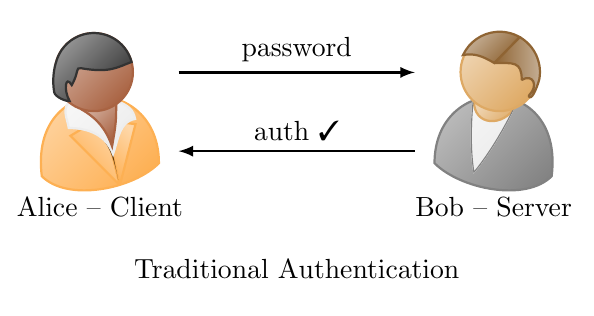
\begin{tikzpicture}[thick,>=latex]
      \node[alice,minimum size=1.5cm] at (0,0) {Alice -- Client};
      \node[bob,mirrored,minimum size=1.5cm] at (5,0) {Bob -- Server};
      \draw[->] (1,0.5) -- (4,0.5) node[midway, above] {password};
      \draw[->] (4,-0.5) -- (1,0-0.5) node[midway, above] {auth \cmark};
      \node at (2.5, -2) {Traditional Authentication};
    \end{tikzpicture}
  \end{figure}
\end{frame}

% talk about how PAKEs are different, state that this is a balanced PAKE
% mention augmented pakes where password is replaced with a verifier
\begin{frame}{Motivation}
  PAKEs are a radically different solution to this problem.
  \begin{itemize}
    \item{the password never leaves a user's device}
    \item{an eavesdropper cannot learn enough information to attack the protocol}
    \item{both the server and client are authenticated with each other}
  \end{itemize}
\end{frame}

\section{Context}

% start talking about how PAKEs work specifically
\begin{frame}{What are PAKEs?}
  \begin{figure}[H]
    \centering
    \begin{tikzpicture}[thick,>=latex]
      \node[alice,minimum size=1.5cm] at (9,0) {Alice -- Client};
      \node[bob,mirrored,minimum size=1.5cm] at (14,0) {Bob -- Server};
      \node at (10.3,0.8) {password};
      \draw[->] (10, 0.5) -- (10,-0.5) node[midway, right, xshift=0.1cm, yshift=0.1cm, scale=0.05] {\includegraphics{wand.png}};
      \node[scale=0.02] at (10.3,-0.7) {\includegraphics{key.png}};
      \node at (12.8,0.8) {password};
      \draw[->] (13, 0.5) -- (13,-0.5) node[midway, left, xshift=-0.1cm, yshift=0.1cm, scale=0.05] {\includegraphics{wand.png}};
      \node[scale=0.02] at (12.5,-0.7) {\includegraphics{key.png}};
      \draw[<->] (10.8,-0.7) -- (12,-0.7) node[midway, below] {auth \cmark};
    \end{tikzpicture}
  \end{figure}
\end{frame}

% talk about example
% talk about replacing the magic with actual maths
\begin{frame}{Example Balanced PAKE}
  \begin{figure}[H]
    \pseudocodeblock[head=SPAKE2]{
      \textbf{Alice} \< \< \textbf{Bob} \\[0.1\baselineskip][\hline]
      \< \< \\[-0.5\baselineskip]
      x \sample \ZZ_p \< \< y \sample \ZZ_p \\
      X \gets g^x \< \< Y \gets g^y \\
      X^* \gets X \cdot M^{pw} \< \< Y^* \gets X \cdot N^{pw} \\
      \< \sendmessageright*{X^*} \< \\
      \< \sendmessageleft*{Y^*} \< \\
      K_A \gets (Y^* / N^{pw})^x \< \< K_B \gets (X^* / M^{pw})^y \\
      SK_A \gets H(A, B, X^*, Y^*, Ka) \< \< SK_B \gets H(A, B, X^*, Y^*, Kb)
    }
  \end{figure}
\end{frame}

% talk about how some more modern cryptographic protocols make use of elliptic curves
\begin{frame}{Elliptic Curves}
  \begin{center}
    \begin{tikzpicture}[thick,>=latex,scale=0.8]
      \begin{scope}
        \draw[<->,gray] (-3,0) -- (3,0) node[right] {$x \in \mathbb{R}$};
        \draw[<->,gray] (0,-3) -- (0,3) node[above] {$y \in \mathbb{R}$};
        \draw[thick, name path=curve, every plot/.style={smooth}] plot[id=weierstrass-curve-1, raw gnuplot] function {
          f(x,y) = y**2 - (x**3 - 2.5*x + 1);
          set xrange [-3:3];
          set yrange [-3:3];
          set view 0,0;
          set isosample 50,50;
          set cont base;
          set cntrparam levels incre 0,0.1,0;
          unset surface;
          splot f(x,y);
        };
      \end{scope}

      \node at (0,-4) {$y^2 = x^3 - 2 x - 1$ over $\mathbb{R}$};
    \end{tikzpicture}
  \end{center}
\end{frame}

% talk about rules
\begin{frame}{Point addition}
  \begin{center}
    \begin{tikzpicture}[scale=.45]
      \begin{scope}[xshift=0cm]
        \plotcurve{-2}{2}
        \draw[->, >=latex, thick] (-2.5,-1) -- ++(0,3.5) node[right] {$\mathcal{O}$};
        \node[below] at (0,-4) {Neutral element $\mathcal{O}$};
      \end{scope}

      \begin{scope}[xshift=7.5cm]
        \plotcurve{-2}{2}
        \draw[dashed, semithick, name path=vertical] (-1.25,2.5) -- ++(0,-5);
        \draw[name intersections={of=curve and vertical}] (intersection-1) node {$\bullet$} node[above left] {$P$}
        (intersection-2) node {$\bullet$} node[below left] {$-P$};
        \node[below] at (0,-4) {Inverse element $-P$};
      \end{scope}

      \begin{scope}[xshift=15cm]
        \plotcurve{-2}{2}
        \draw[thick, name path=chord] (-2.5,.5) -- (2.5,2.0);
        \draw[name intersections={of=curve and chord}] (intersection-1) node {$\bullet$} node[above left] {$P$}
        (intersection-2) node {$\bullet$} node[above right=-1pt] {$Q$}
        (intersection-3) node {$\bullet$} coordinate[name=mPQ];
        \draw[dashed, semithick, name path=vertical] (mPQ) ++(0,1) -- +(0,-5.5);
        \draw[name intersections={of=curve and vertical}] (intersection-2) node {$\bullet$} node[below left] {$P+Q$};
        \node[below, align=center] at (0,-4) {Addition $P+Q$ \\ ``Chord rule''};
      \end{scope}

      \begin{scope}[xshift=22.5cm]
        \plotcurve[thick, tangent=0.265, every plot/.style={sharp plot}]{-2}{2}
        \draw[thick, use tangent, name path=chord] (-.6,0) -- (1.5,0);
        \draw[name intersections={of=curve and chord}] (intersection-1) node {$\bullet$} node[above] {$P$}
        (intersection-2) node {$\bullet$} coordinate[name=mPQ];
        \draw[dashed, semithick, name path=vertical] (mPQ) ++(0,1) -- +(0,-5.0);
        \draw[name intersections={of=curve and vertical}] (intersection-2) node {$\bullet$} node[below left] {$2P$};
        \node[below, align=center] at (0,-4) {Doubling $P+P$ \\ ``Tangent rule''};
      \end{scope}

    \end{tikzpicture}
  \end{center}
\end{frame}

% Talk about how computers cannot operate on real numbers
% instead we have to bound the numbers somehow, and we use the finite field of integers mod some prime p
\begin{frame}{Finite Fields}
	\begin{alertblock}{Computers cannot represent the real numbers.\\}
    Instead a finite set must be chosen instead.\\
    The Finite Field of integers mod some prime $p$ is used instead of the reals.
	\end{alertblock}

  This is notated $\FF_p$, $\text{GF}(p)$.
\end{frame}

\begin{frame}{Elliptic Curves Over Finite Fields}
  \begin{figure}[H]
    \centering
    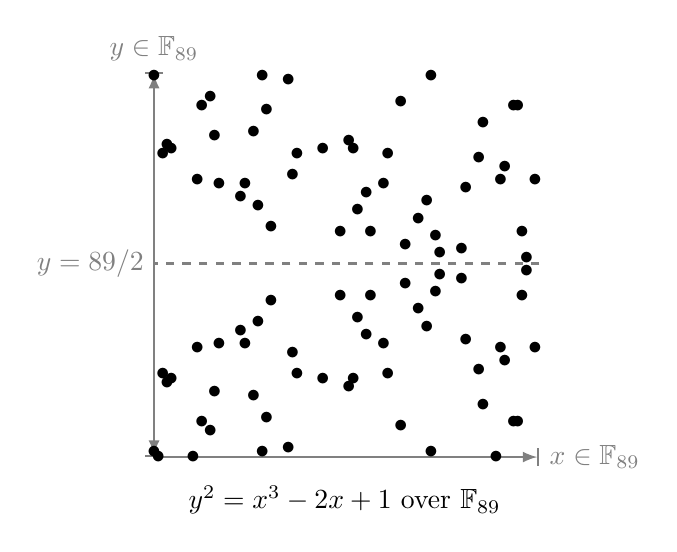
\begin{tikzpicture}[thick,>=latex]
      % Generate list of points with Sage:
      % sage: E = EllipticCurve(Integers(89), [-2,1])
      % sage: points = {tuple(p)[:2] for p in E.points()}
      % sage: print(points)
      \begin{scope}[scale=.055]
        \draw[|<->|,gray] (0,0) -- (0,89) node[above] {$y \in \mathbb{F}_{89}$};
        \draw[->|,gray] (0,0) -- (89,0) node[right] {$x \in \mathbb{F}_{89}$};
        % weirdness to make the line actually split the plane
        \draw[dashed,gray] (89,44.7) -- (0,44.7) node[left] {$y = 89/2$};
        \foreach \point in {
          (43, 37), (50, 52), (72, 27), (20, 29), (58, 40), (58, 49), (14, 15), (27, 36), (13, 83), (26, 80), (47, 57), (65, 38), (3, 72), (3, 17), (24, 58), (33, 70), (26, 9), (84, 8), (54, 19), (45, 16), (85, 52), (14, 74), (4, 18), (75, 69), (45, 73), (65, 51), (86, 46), (49, 61), (33, 19), (81, 22), (39, 71), (25, 88), (9, 0), (79, 0), (50, 37), (2, 70), (53, 63), (20, 60), (27, 53), (39, 18), (84, 81), (31, 87), (43, 52), (80, 25), (1, 0), (25, 1), (15, 63), (76, 12), (64, 1), (63, 30), (66, 47), (80, 64), (83, 8), (72, 62), (88, 25), (2, 19), (21, 63), (23, 14), (21, 26), (64, 88), (32, 65), (71, 48), (88, 64), (81, 67), (10, 25), (31, 2), (0, 88), (85, 37), (66, 42), (61, 55), (53, 26), (71, 41), (10, 64), (11, 8), (75, 20), (11, 81), (32, 24), (54, 70), (15, 26), (49, 28), (0, 1), (83, 81), (57, 7), (86, 43), (46, 71), (24, 31), (23, 75), (4, 71), (47, 32), (76, 77), (13, 6), (63, 59), (46, 18), (61, 34), (57, 82)
        } {\node at \point {$\bullet$};}
        \node at (44,-10) {$y^2 = x^3 - 2 x + 1$ over $\mathbb{F}_{89}$};
      \end{scope}
    \end{tikzpicture}
  \end{figure}
\end{frame}

\begin{frame}{AuCPace}
  An Augmented PAKE designed for the Industrial Internet of Things (IIOT).
  \begin{itemize}
    \item{Proved secure in the Universal Composability framework}
    \item{Optimised to run efficiently on small microcontrollers}
    \item{
      Three variants to allow users to adapt the protocol to their setting:
      \begin{itemize}
        \item{Strong AuCPace -- provides pre-computation resistance by blinding the salt value}
        \item{Partial Augmentation -- server stores a long term keypair for each user}
        \item{Implicit Mutual Authentication -- removes a round of messages}
      \end{itemize}
    }
  \end{itemize}
\end{frame}

\begin{frame}{RustCrypto}
  \begin{center}
    \includegraphics[width=0.9\linewidth]{rust_crypto_github.png}
  \end{center}
\end{frame}

\section{Demo}

\begin{frame}{Conclusion}
  I have implemented the AuCPace protocol and all it's variants in an ergonomic Rust libary.\\
  The library has been open-sourced through the RustCrypto.
\end{frame}

\begin{frame}[standout]
  Thank you for watching!
\end{frame}

\end{document}
